\documentclass[12 pt,a4paper,french]{article}

\usepackage{babel}

\usepackage{graphicx}
\graphicspath{{images/}}

\usepackage{url}
\usepackage{csquotes}
\usepackage[backend=biber,style=numeric]{biblatex}
 \addbibresource{rapport.bib}

\usepackage[T1]{fontenc}
\usepackage{fontspec}

\title{Rapport du projet MyAdblock}

\author{Adam FACI \\ Quentin DECHAUX}

\begin{document}

\begin{titlepage}
  
\includegraphics[scale = 0.7]{TNCY.jpg}
  
\includegraphics[scale = 1.5]{UL.jpg}
  \vspace{3 cm}

  \begin{center}
    \textbf{\Huge{\maketitle}}
    \vspace{1 cm}
  \end{center}
  \vfill
  \textbf{Cours :} Réseaux et Systèmes Avancés : Partie Réseaux\\
  \textbf{Professeur :} Isabelle CHRISMENT
\end{titlepage}

\tableofcontents
\thispagestyle{empty}

\newpage
\setcounter{page}{1}

\section{Introduction}

\hspace{5mm}Projet effectué dans le cadre du cours de RSA visant à comprendre la notion de serveur proxy HTTP en créant le nôtre et en l'utilisant en tant que ``AdBlock'' ie. en tant que bloqueur de publicités.\\\par

Le serveur devra à chaque requête arrivant sur notre machine vérifier que l'hôte de celle-ci ne fait pas partie d'une liste prédéfinie de serveurs de publicités.\\\par

À priori la liste proviendra du site \url{https://easylist.to/}.

\section{Question 1}

\hspace{5mm}Les échanges TCP et HTTP entre le client (notre machine) et le serveur web (le site \url{www.telecomnancy.eu}) ont été triés via le filtre : ``(tcp || http) \&\& ip.addr == 193.50.135.38'' où ``193.50.135.38'' correspond à l'adresse ip du site au moment de la communication.\\\par

Le résultat de ces échanges sont en pièce jointe dans le fichier ``capture\_file\_question\_1.pcapng''.\\\par

Cela commence tout d'abord avec un \textcite{1}``TCP three-way handshake'' avec le serveur qui reçoit le segment SYN, nous qui recevons le segment SYN+ACK et enfin le serveur qui reçoit le segment ACK.

\begin{figure}
  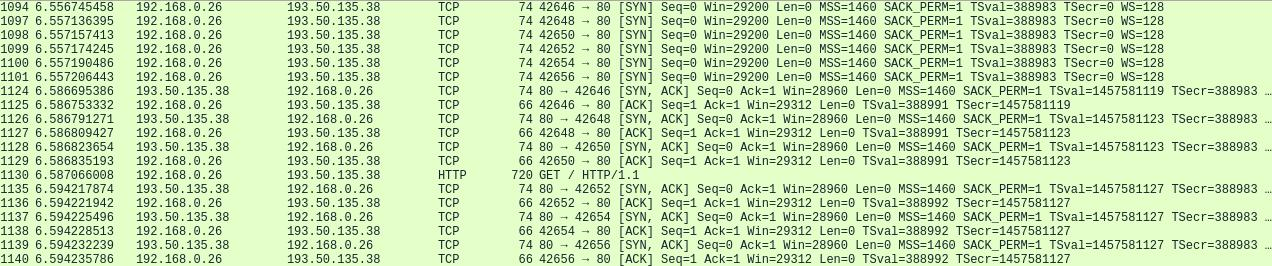
\includegraphics[height=7cm,width=20cm]{three_way_handshake.jpg}
  \caption{Le three-way handshake}
\end{figure}
\printbibliography
\end{document}